\label{sec:results}

In this Section, the unfolded distributions of the 
averge jet mass
are investigated.
In Figures~\ref{figs:unfoldedMeasurementDijets_1_allsys}-
\ref{figs:unfoldedMeasurementDijets_9_Pruned_allsys}, 
the differential cross
section from Eq.~\ref{eq:pdf_mjet_simple} is shown for
various $\pt^{AVG}$ bins, as a function of
$m_{J}^{AVG}$, as described in
Section~\ref{sec:dataSampleAndEventSelection}, 
for ungroomed jets and for different grooming algorithms. 
As described in Eq.~\ref{eq:pdf_mjet_simple},
each distribution in each $\pt^{AVG}$ is separately normalized to
unity, and each bin content is divided by the bin width of the
$m_J^{AVG}$ bin,
so these plots show the probability distribution function of $m_J^{AVG}$,
with units of 1/GeV (see Eq.~\ref{eq:pdf_mjet_simple}. 
The shapes for $m_J^{AVG}$ in the MC samples are
taken directly from the MC. The bias correction described in
Section~\ref{sec:closure} is also applied. 


The statistical uncertainty is shown in light yellow, the
uncertainties due to the jet-energy resolution, jet-energy scale, and
jet-angular resolution are shown in shades of brown, the uncertainty
due to pile-up is shown in green, and the uncertainty due to the
parton shower differences are shown in dark yellow,
and the uncertainty due to closure bias correction is shown in gray.
The simulated distribution from \PYTHIA is shown in solid black, 
the from \PYTHIAEIGHT in dashed red, and from \HERWIG in dotted blue. 
The bottom frame shows the ratio of the true distribution from
the simulation divided by the unfolded distribution, along with
the uncertainties in the unfolded distribution. 

Due to an artifact of the binning, combined with the strategy of
subtracting two PDFs to obtain the uncertainty on the parton shower
model, oftentimes the difference between the PDFs is close to zero in
a single bin. In order to avoid unphysical regions of the uncertainty
bands, the uncertainty bands are averaged in regions where the
uncertainty bands are very close to zero, by averaging adjacent bins. 
This is implemented technically by replacing the uncertainty of bins
by the adjacent-bin averaged value,
when the systematic uncertainty is at a local minimum, and is less
than 4\% of the central value. 

Figures~\ref{figs:unfoldedMeasurementDijets_1}-
\ref{figs:unfoldedMeasurementDijets_9_Pruned}, 
show the same plots, however in a simplified format with only the
total and statistical uncertainties shown in dark yellow and 
light yellow, respectively. 


As a summary of the information in each bin, several of the
$\pt^{AVG}$ bins are shown in
Figures~\ref{figs:unfoldedMeasurementDijets_all},
\ref{figs:unfoldedMeasurementDijets_all_Filtered},
\ref{figs:unfoldedMeasurementDijets_all_Trimmed},
and 
\ref{figs:unfoldedMeasurementDijets_all_Pruned},
for AK7 jets with no grooming, filtering, trimming, and pruning 
applied, respectively. 
Figures~\ref{figs:unfoldedMeasurementDijets_allfrac},
\ref{figs:unfoldedMeasurementDijets_allfrac_Filtered},
\ref{figs:unfoldedMeasurementDijets_allfrac_Trimmed},
and 
\ref{figs:unfoldedMeasurementDijets_allfrac_Pruned},
show the ratio of MC truth to the data, for 
\PYTHIA, \HERWIG, and \PYTHIA8 for all of the
grooming cases. 

\subsection{Discussion}

The agreement with the \HERWIG parton-shower model seems to be the
best for $\pt^{AVG} > 300$ \GeVc. Above $\pt^{AVG} > 300$ \GeV, the 
\HERWIG model seems to describe the jet mass very well above
$m_{J}^{AVG} > 50$ \GeVcc. After applying the various grooming techniques,
the agreement is even improved, and the agreement begins
at around $m_{J}^{AVG} > 20$ \GeVcc. However, the filtering
algorithm seems to have slightly worse agreement again 
for $20 < m_{J}^{AVG} < 50$ \GeVcc and $\pt^{AVG} > 450$ \GeVc.

For all of the generators and all of the $\pt^{AVG}$ bins, 
the agreement gets better for
larger jet masses. At the very lowest jet masses, the disagreement
is the largest. 

The largest systematic effect is the difference in the
unfolding using different parton shower models, with
subleading, but still significant, uncertainties due to
jet energy scale and resolution, and
small contributions from jet angular resolution and pileup. 


\begin{figure}[htbp]
\centering
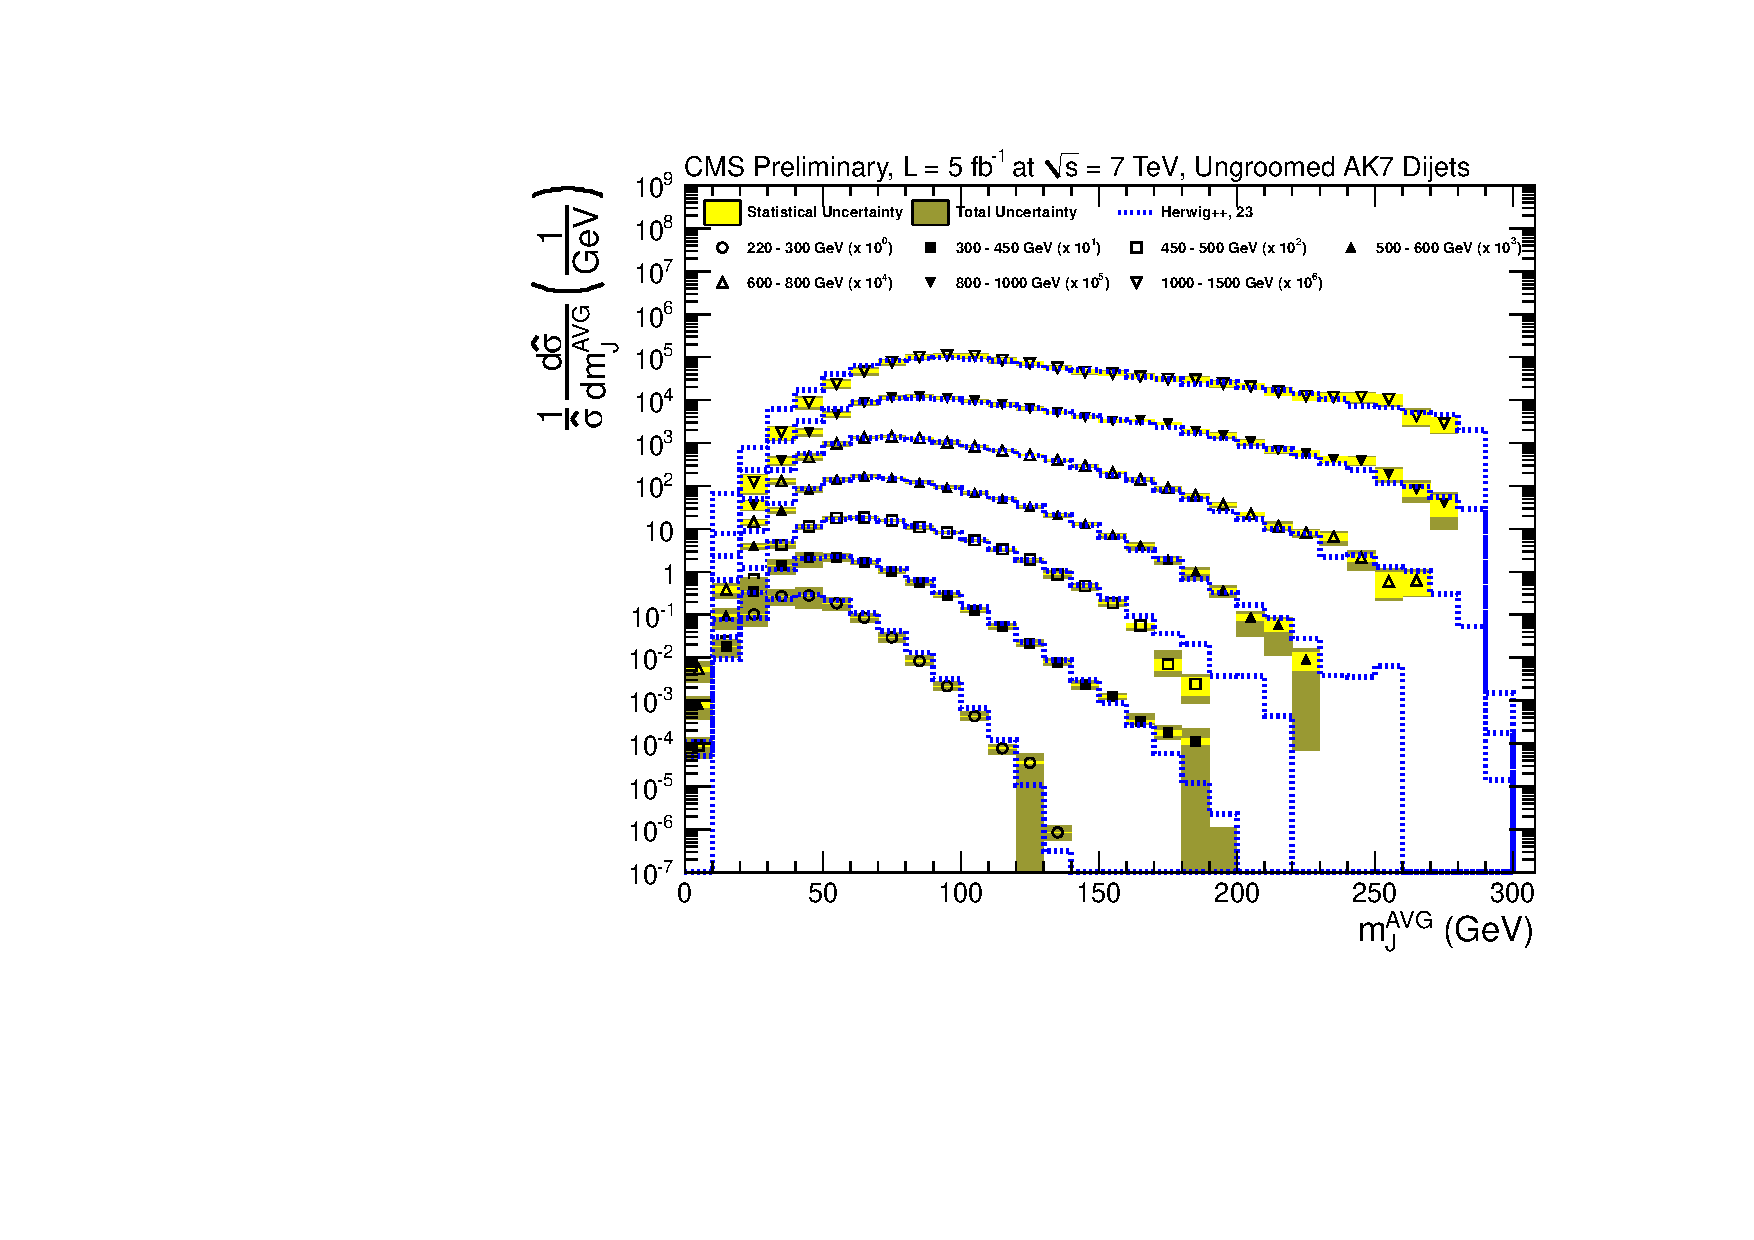
\includegraphics[width=0.95\textwidth]{figs/unfoldedMeasurementDijets_all_}
\caption{Unfolded distributions of the jet mass for AK7 jets,
The data are shown in black points. 
The statistical uncertainty is shown in light yellow, and the
systematic uncertainty is shown in dark yellow.
The higher $\pt^{AVG}$ bins are scaled by a factor to
enhance visibility.
\label{figs:unfoldedMeasurementDijets_all}}
\end{figure}

\begin{figure}[htbp]
\centering
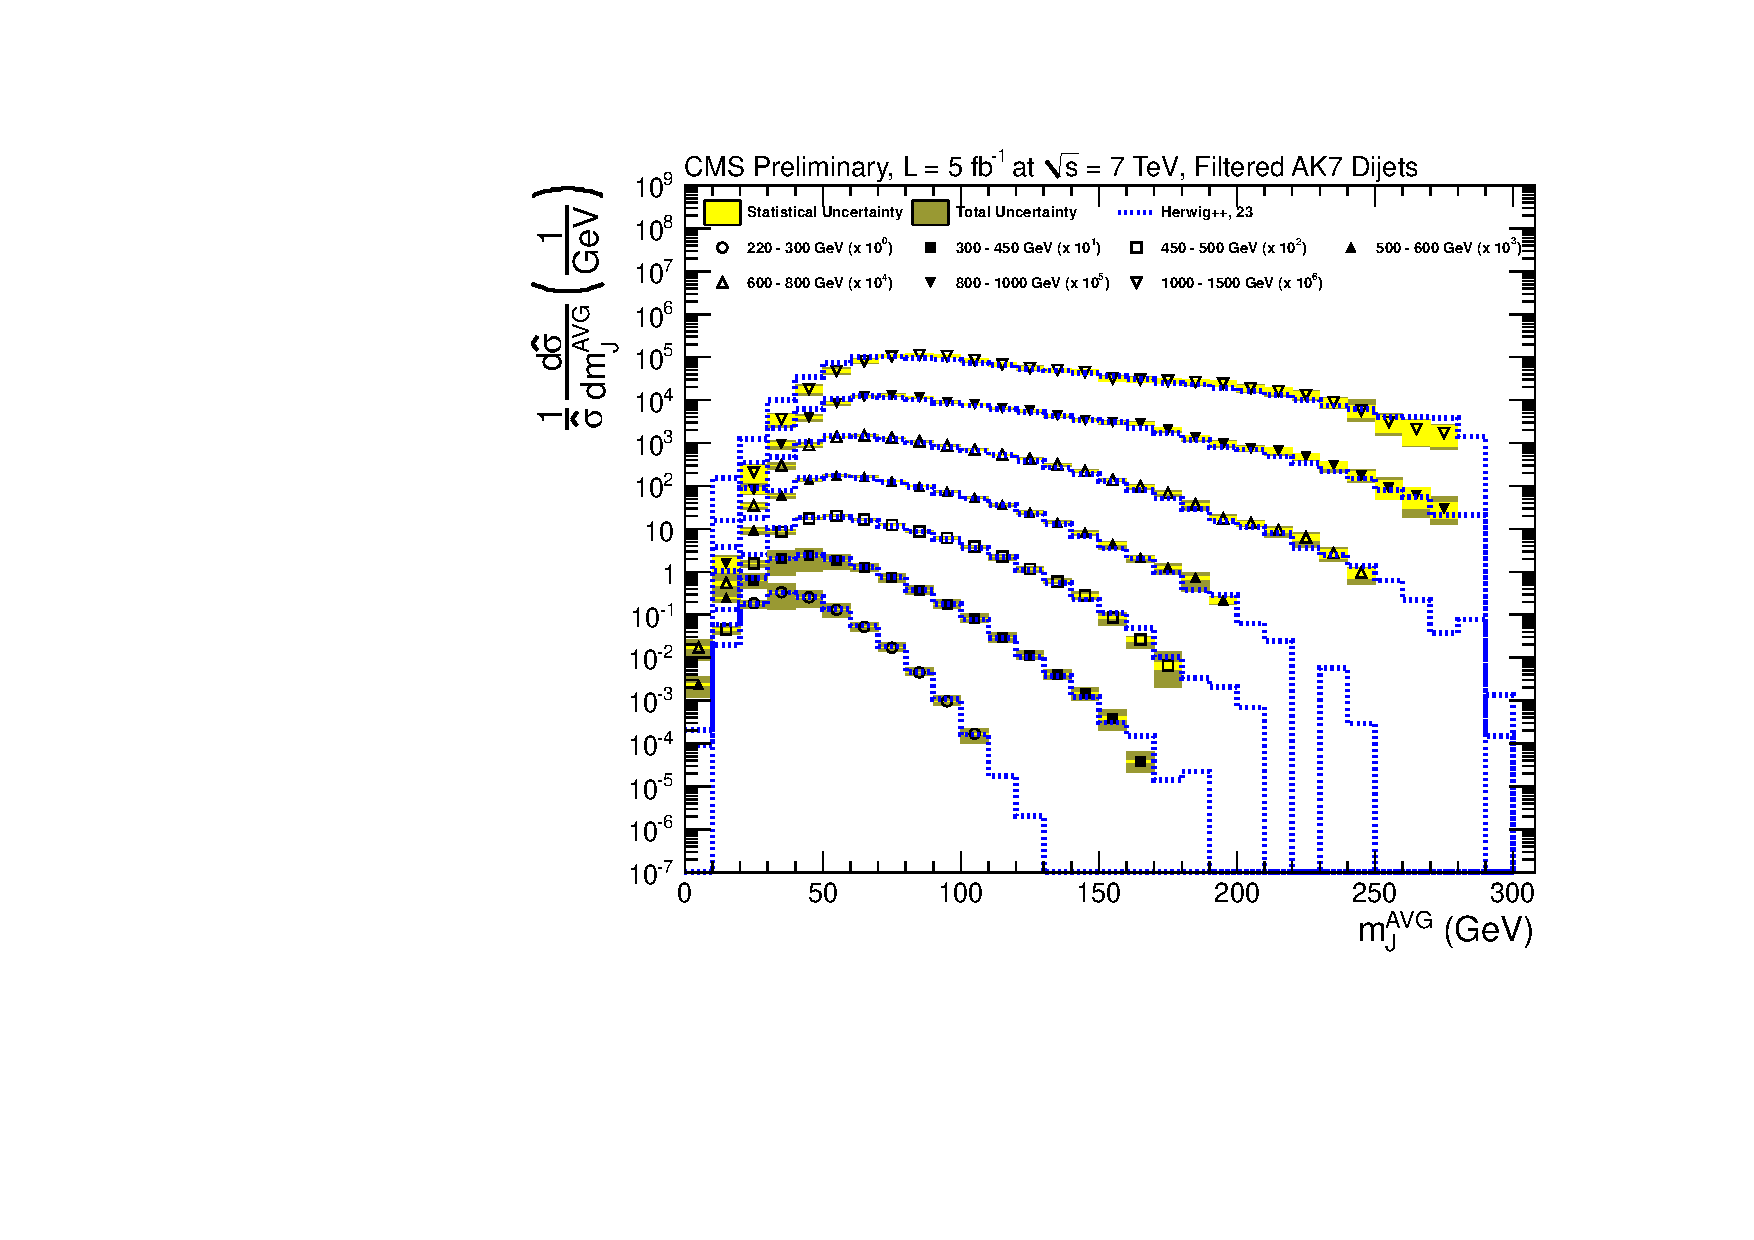
\includegraphics[width=0.95\textwidth]{figs/unfoldedMeasurementDijets_all__Filtered}
\caption{Unfolded distributions of the jet mass for filtered AK7 jets,
The data are shown in black points. 
The statistical uncertainty is shown in light yellow, and the
systematic uncertainty is shown in dark yellow.
The higher $\pt^{AVG}$ bins are scaled by a factor to
enhance visibility.
\label{figs:unfoldedMeasurementDijets_all_Filtered}}
\end{figure}

\begin{figure}[htbp]
\centering
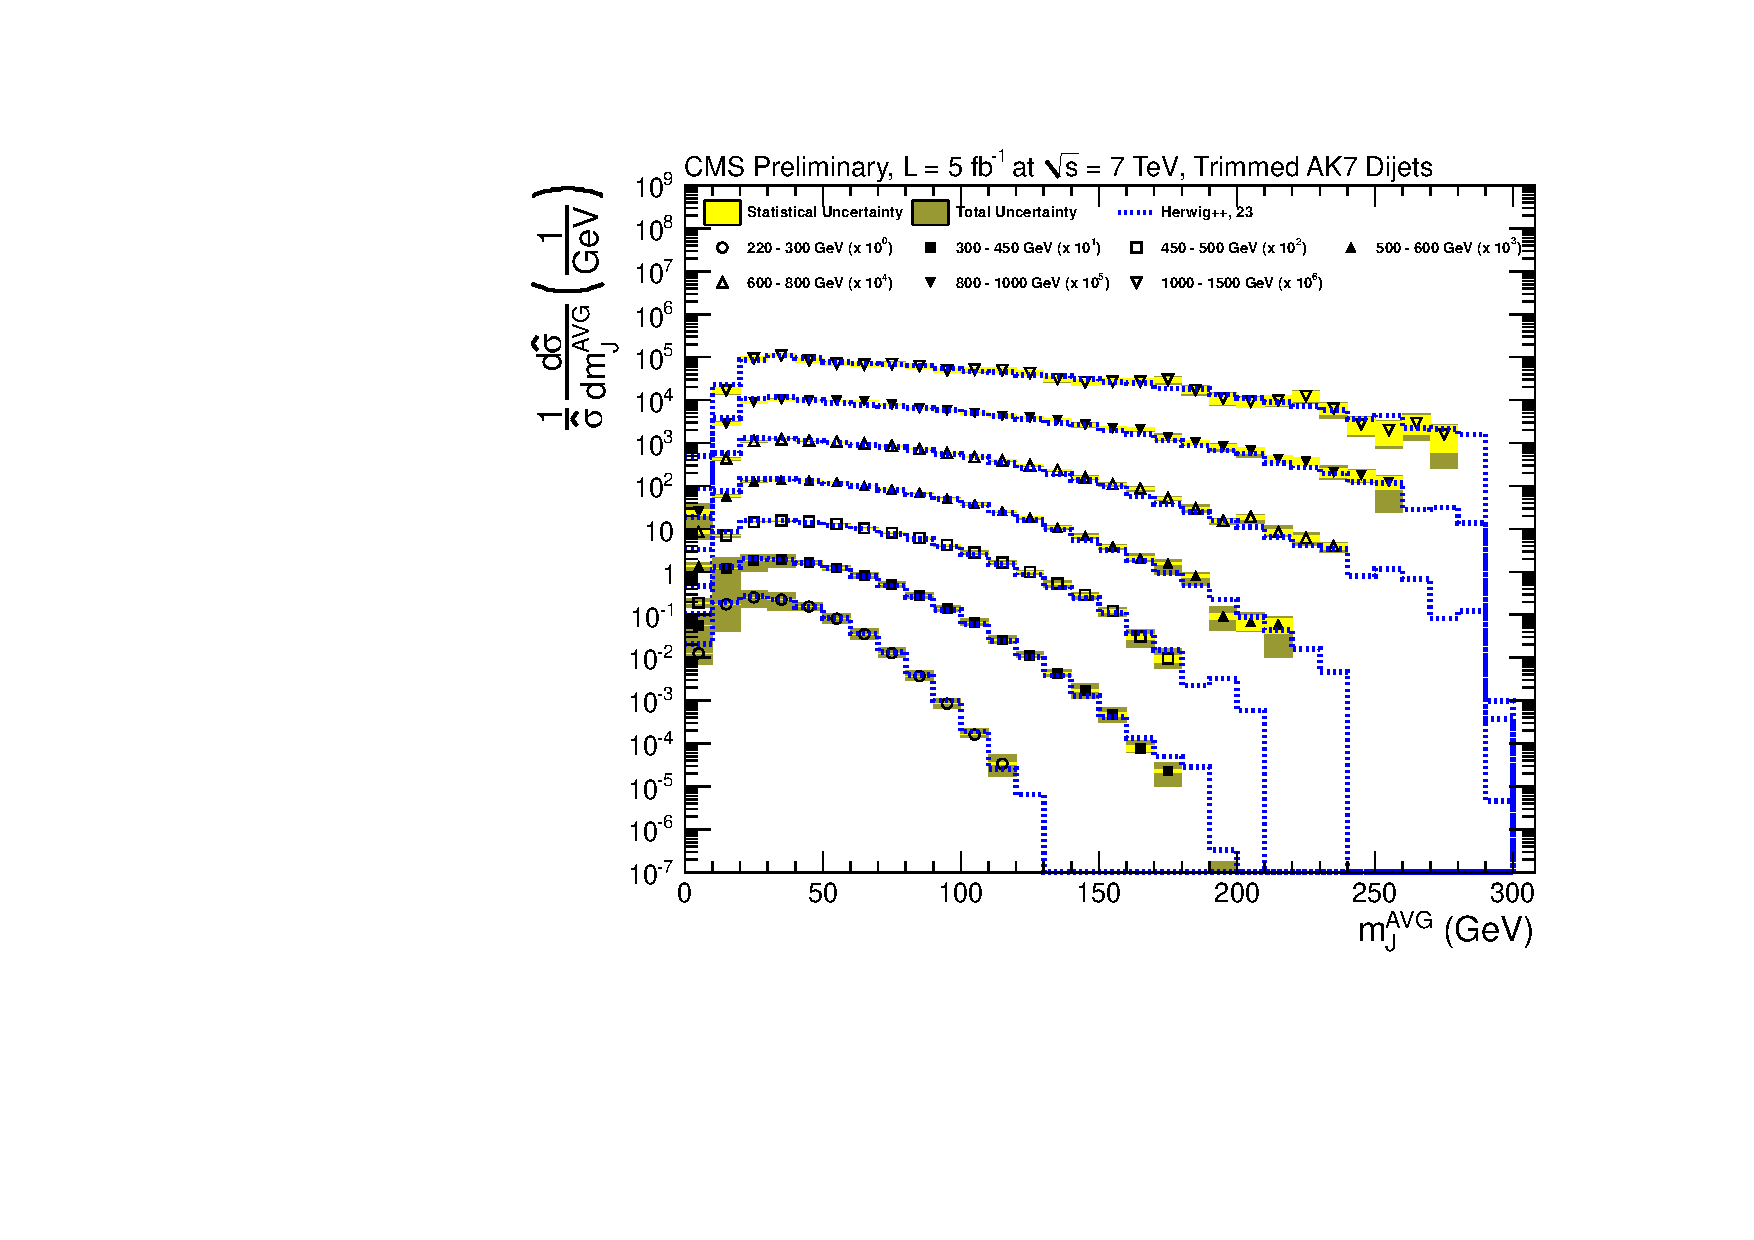
\includegraphics[width=0.95\textwidth]{figs/unfoldedMeasurementDijets_all__Trimmed}
\caption{Unfolded distributions of the jet mass for trimmed AK7 jets,
The data are shown in black points. 
The statistical uncertainty is shown in light yellow, and the
systematic uncertainty is shown in dark yellow.
The higher $\pt^{AVG}$ bins are scaled by a factor to
enhance visibility.
\label{figs:unfoldedMeasurementDijets_all_Trimmed}}
\end{figure}

\begin{figure}[htbp]
\centering
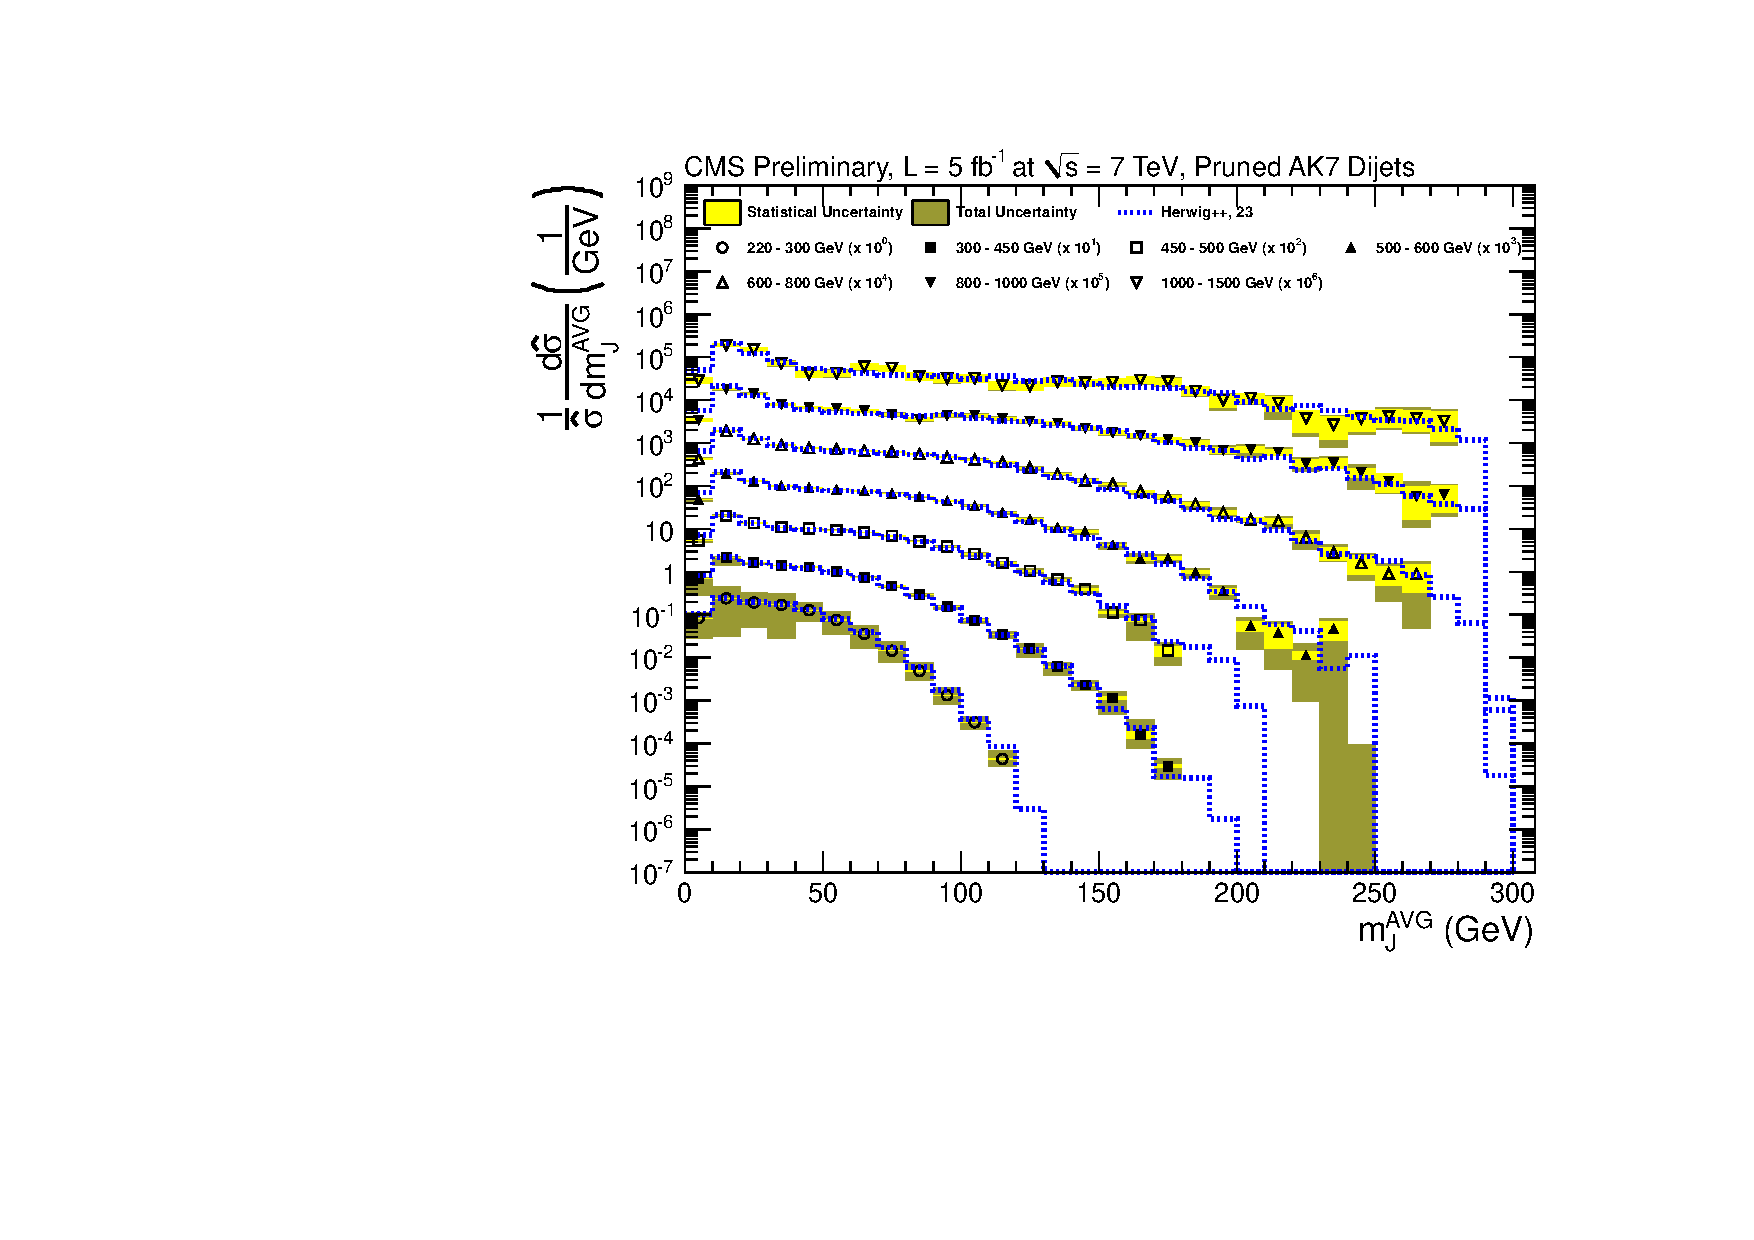
\includegraphics[width=0.95\textwidth]{figs/unfoldedMeasurementDijets_all__Pruned}
\caption{Unfolded distributions of the jet mass for pruned AK7 jets,
The data are shown in black points. 
The statistical uncertainty is shown in light yellow, and the
systematic uncertainty is shown in dark yellow.
The higher $\pt^{AVG}$ bins are scaled by a factor to
enhance visibility.
\label{figs:unfoldedMeasurementDijets_all_Pruned}}
\end{figure}




\begin{figure}[htbp]
\centering
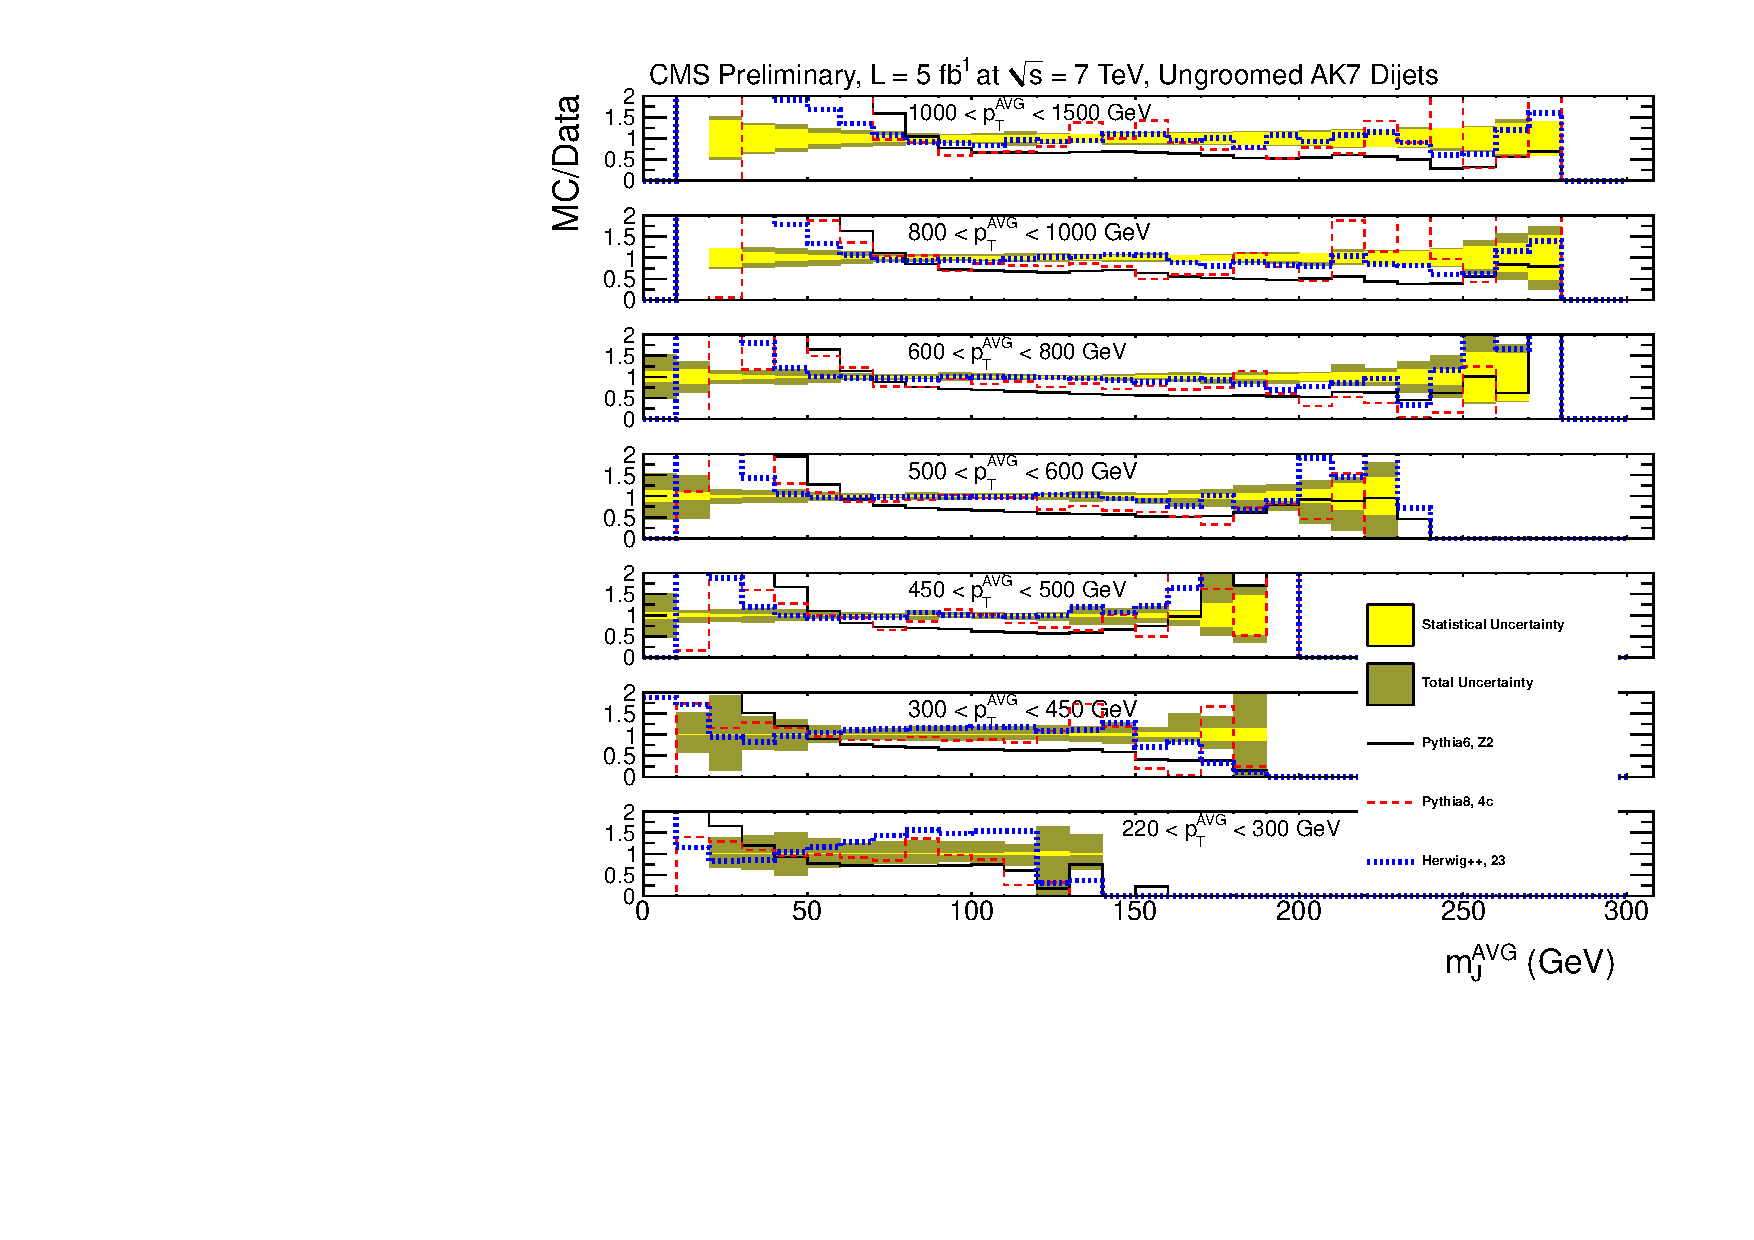
\includegraphics[width=0.95\textwidth]{figs/unfoldedMeasurementDijets_allfrac_}
\caption{Ratio of MC truth to unfolded distributions of the jet mass for AK7 jets,
The data are shown in black points. 
The statistical uncertainty is shown in light yellow, and the
systematic uncertainty is shown in dark yellow. \PYTHIA is shown in solid black, \HERWIG is shown in dotted blue, and \PYTHIA8 is shown in dashed red.
\label{figs:unfoldedMeasurementDijets_allfrac}}
\end{figure}

\begin{figure}[htbp]
\centering
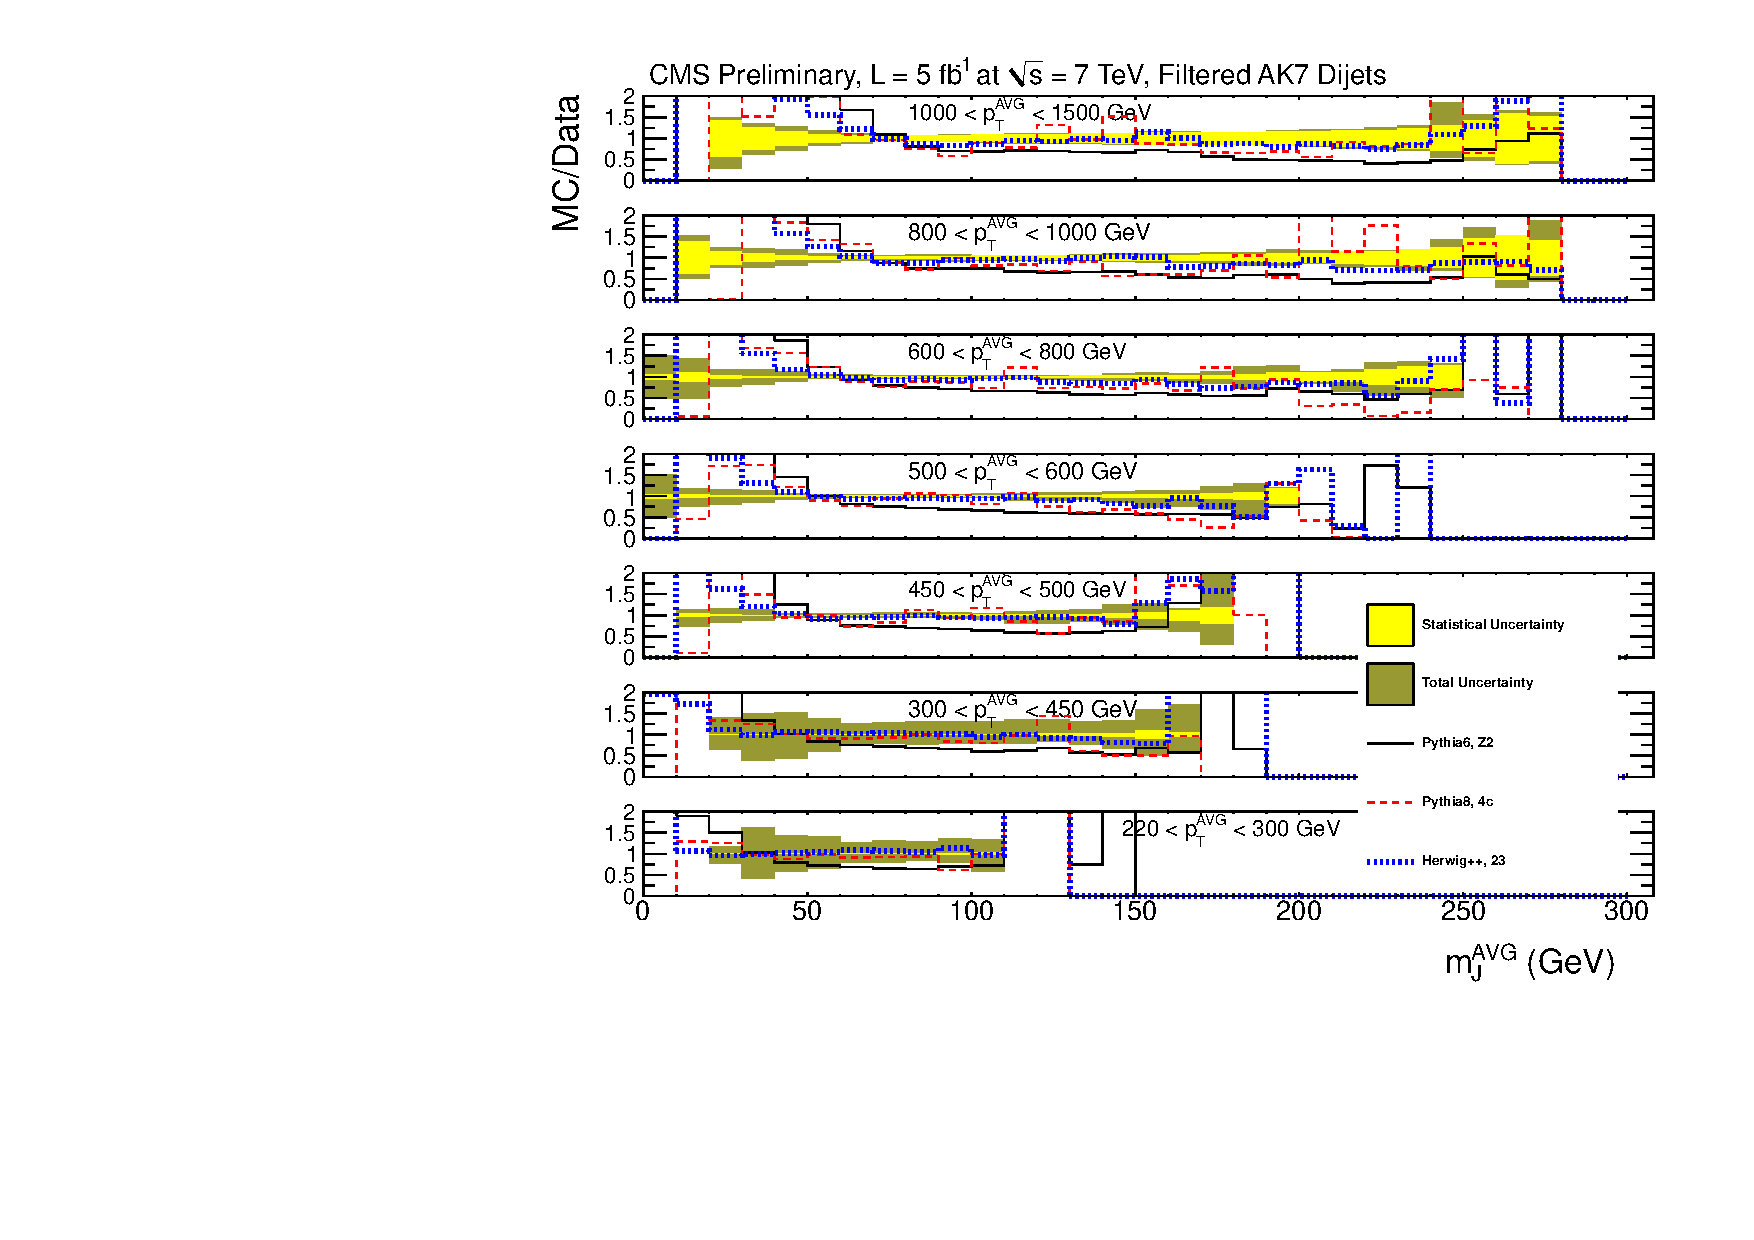
\includegraphics[width=0.95\textwidth]{figs/unfoldedMeasurementDijets_allfrac__Filtered}
\caption{Ratio of MC truth to unfolded distributions of the jet mass for filtered AK7 jets,
The data are shown in black points. 
The statistical uncertainty is shown in light yellow, and the
systematic uncertainty is shown in dark yellow. \PYTHIA is shown in solid black, \HERWIG is shown in dotted blue, and \PYTHIA8 is shown in dashed red.
\label{figs:unfoldedMeasurementDijets_allfrac_Filtered}}
\end{figure}

\begin{figure}[htbp]
\centering
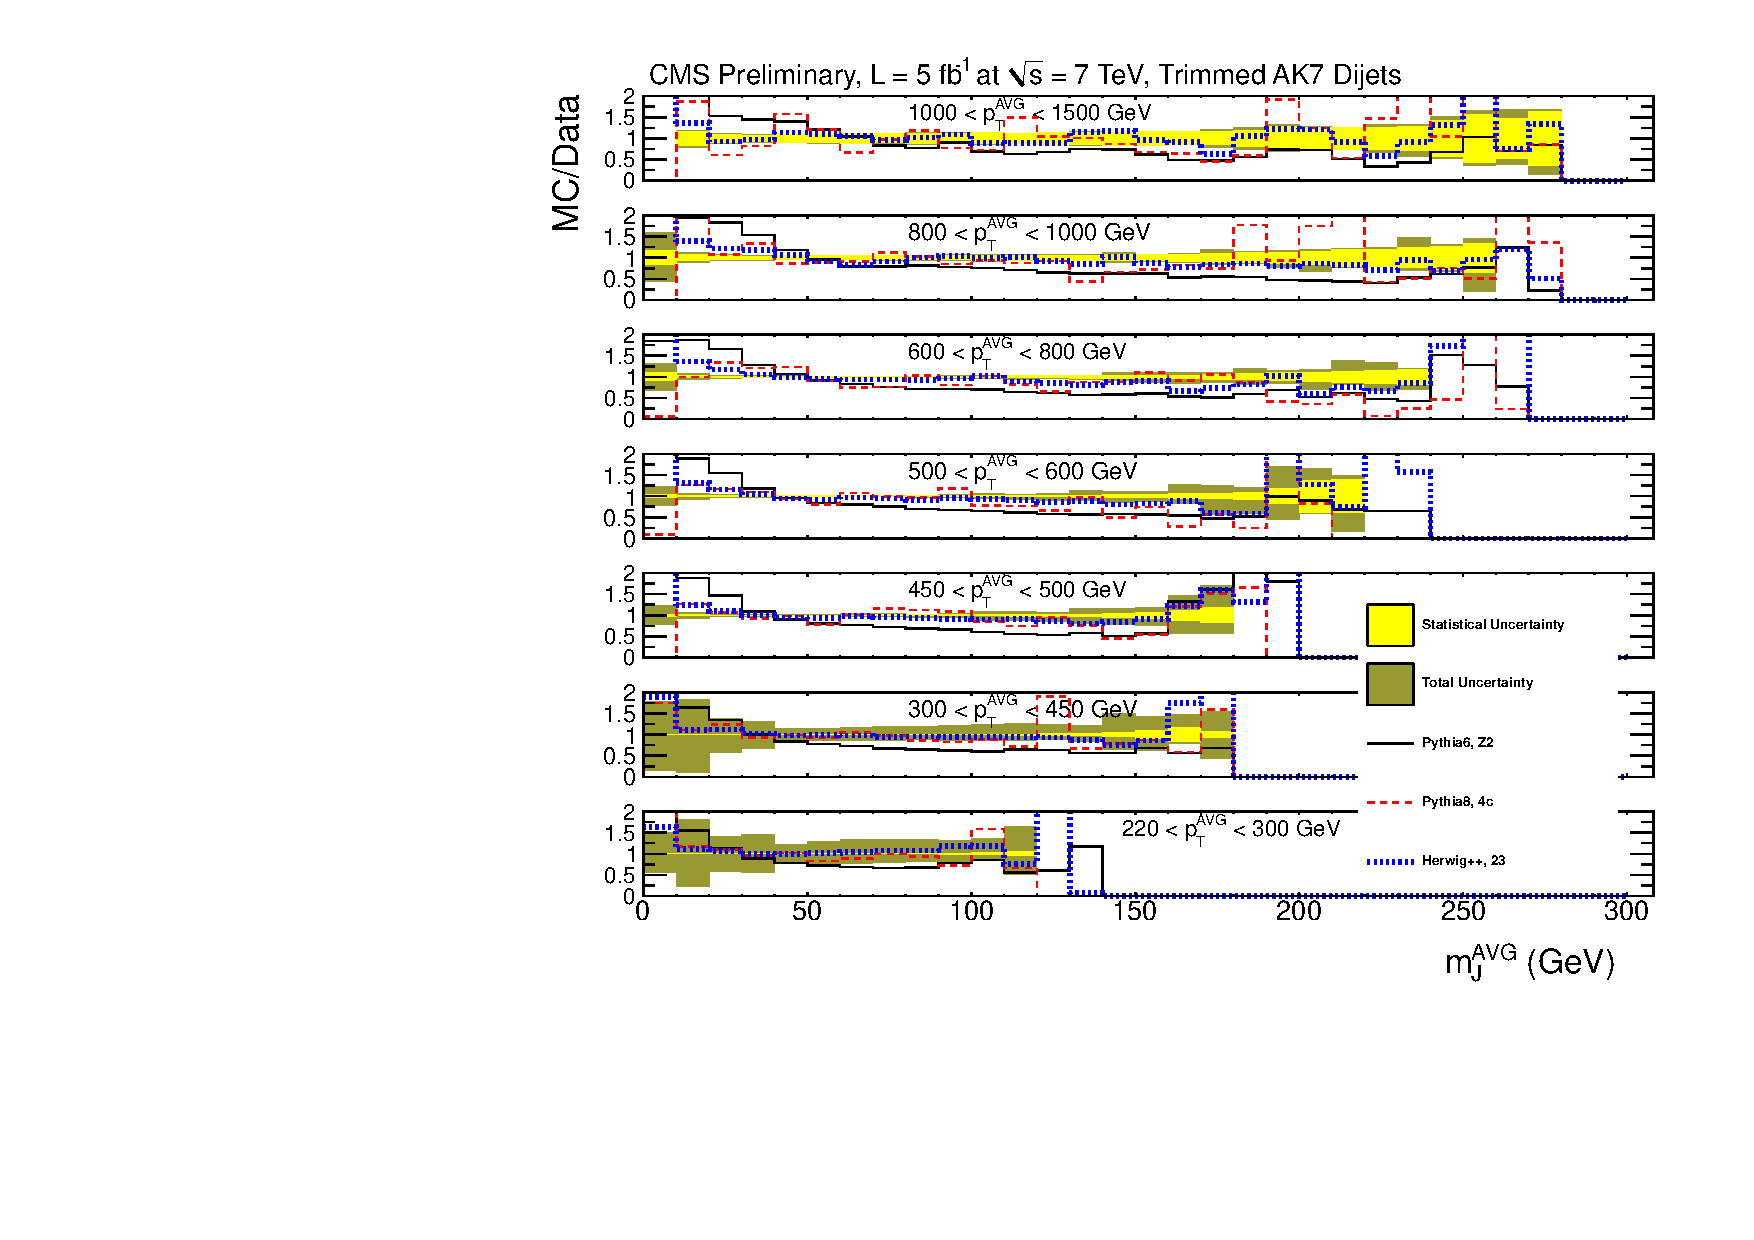
\includegraphics[width=0.95\textwidth]{figs/unfoldedMeasurementDijets_allfrac__Trimmed}
\caption{Ratio of MC truth to unfolded distributions of the jet mass for trimmed AK7 jets,
The data are shown in black points. 
The statistical uncertainty is shown in light yellow, and the
systematic uncertainty is shown in dark yellow. \PYTHIA is shown in solid black, \HERWIG is shown in dotted blue, and \PYTHIA8 is shown in dashed red.
\label{figs:unfoldedMeasurementDijets_allfrac_Trimmed}}
\end{figure}

\begin{figure}[htbp]
\centering
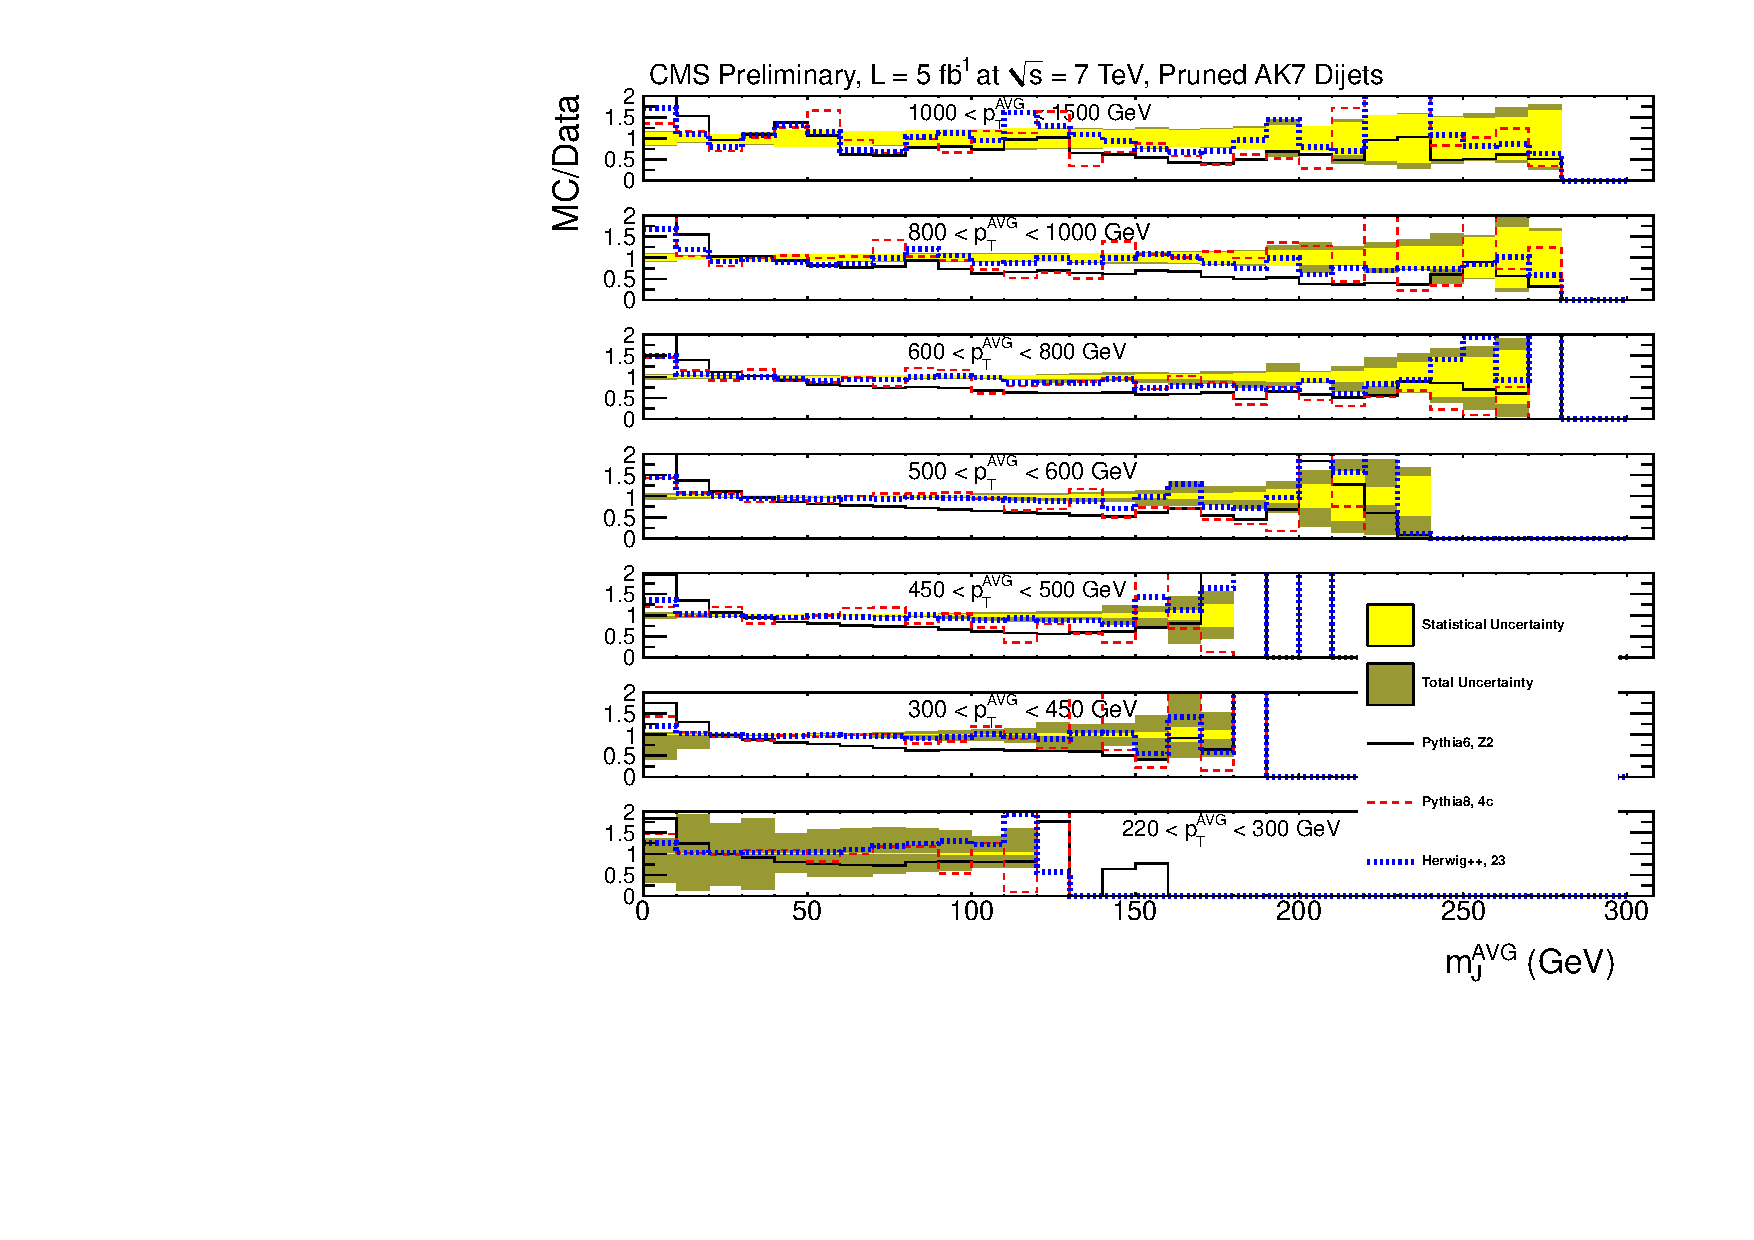
\includegraphics[width=0.95\textwidth]{figs/unfoldedMeasurementDijets_allfrac__Pruned}
\caption{Ratio of MC truth to unfolded distributions of the jet mass for pruned AK7 jets,
The data are shown in black points. 
The statistical uncertainty is shown in light yellow, and the
systematic uncertainty is shown in dark yellow. \PYTHIA is shown in solid black, \HERWIG is shown in dotted blue, and \PYTHIA8 is shown in dashed red.
\label{figs:unfoldedMeasurementDijets_allfrac_Pruned}}
\end{figure}



\subsection{Cross-check with bin-by-bin unfolding}

As a cross-check of the unfolding procedure, a bin-by-bin unfolding
method is used. The unfolded summary plots for the ungroomed AK7 jets
are shown in Fig.~\ref{figs:unfoldedMeasurementDijetsbinbybin_all}.
There are a few places where the bin-by-bin unfolding fails which is
one shortcoming of the method anyway, but
overall there is good agreement with the Bayesian unfolding in the
results where expected.


\begin{figure}[htbp]
\centering
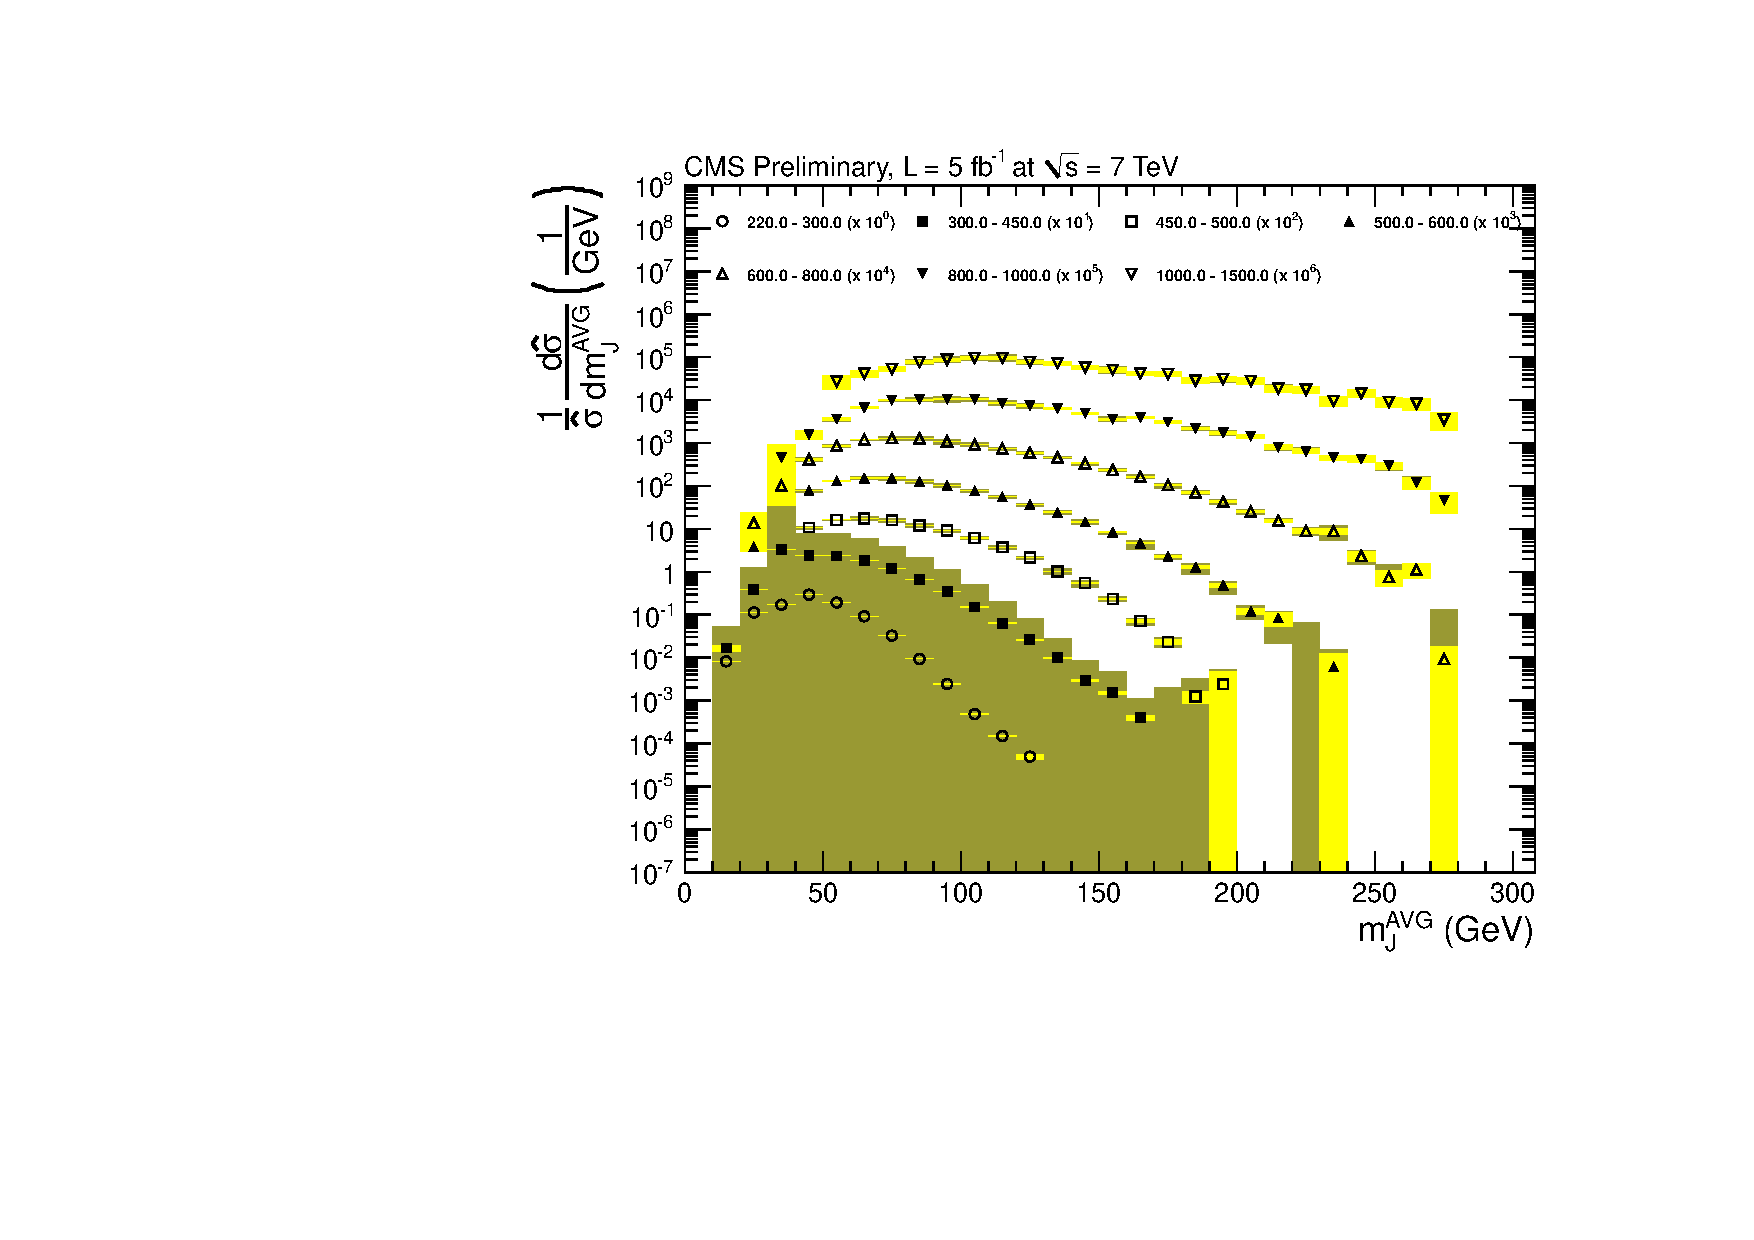
\includegraphics[width=0.95\textwidth]{figs/unfoldedMeasurementDijets_all_binbybin}
\caption{Unfolded distributions of the jet mass for AK7 jets,
using a cross-check unfolding procedure of bin-by-bin unfolding.
The data are shown in black points. 
The statistical uncertainty is shown in light yellow, and the
systematic uncertainty is shown in dark yellow.
The higher $\pt^{AVG}$ bins are scaled by a factor to
enhance visibility.
\label{figs:unfoldedMeasurementDijetsbinbybin_all}}
\end{figure}
